\subsection {Unpacking raw data from the camera}
\label{sec:unpacking}


The \lucid cameras feature a 12-bit \gls{adc} and offer 23 different output formats with varying bit depths and packing.
As the \gls{h265} encoder supports up to 10-bit input, the \code{Mono10p} output format was chosen for the cameras \cite[17 ]{nvidiaNVIDIAJetsonAGX2019}
This format densly packs the 10-bit data, as depicted in Figure \ref{fig:mono10p}, maximizing the network throughput.

\begin{figure}[H]
    \centering
    \subcaptionbox{Pixel data.}{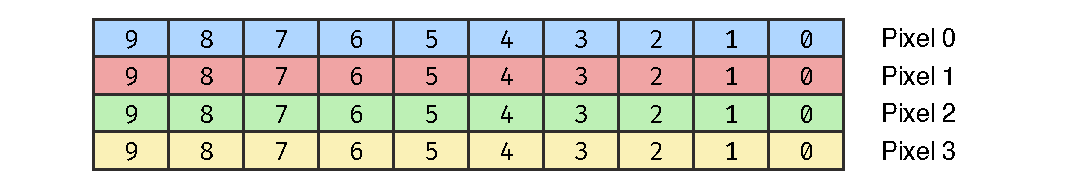
\includegraphics[width=\textwidth]{figures/unpacking/layout_10p.pdf}}
    \subcaptionbox{Bytes sent over ethernet.}{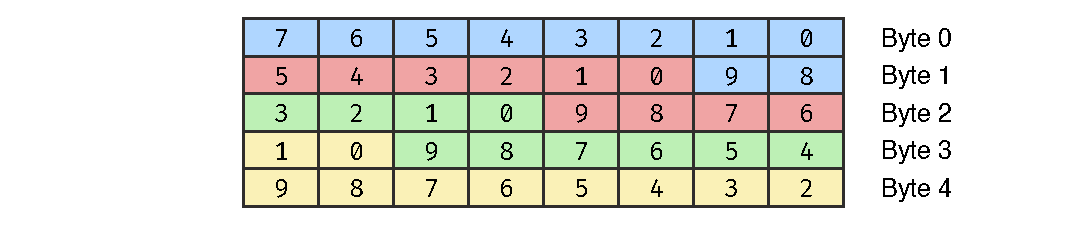
\includegraphics[width=\textwidth]{figures/unpacking/layout_10p_sent.pdf}}
    \caption{Bit layout of the \code{Mono10p} format.}
    \label{fig:mono10p}
\end{figure}


I encountered difficulties in locating documentation regarding the bit ordering on Lucid's website.
As a workaround, I relied on two test images provided by the \cam.
These test images contained pixel values that increased monotonically, as depicted in Figure \ref{fig:test_pattern}.
By analyzing the data in the first line these images, I was able to deduce the bit ordering.
Regrettably, I later discovered that Lucid Vision does provide documentation on pixel formats; however, it did not appear in their own search engine for unknown reasons \cite{lucidvisionlabsPixelFormatsLUCID2020}.

\begin{figure}[H]
    \centering
    
\includegraphics[width=0.4\textwidth]{figures/unpacking/test_pattern0.jpg}
    
\includegraphics[width=0.4\textwidth]{figures/unpacking/test_pattern2.jpg}
    \caption{Two test images used to infer the bit ordering.
        The \cam can output several different test patterns useful for various testing purposes \cite{lucidvisionlabsTritonMPPolarized2020}.}
    \label{fig:test_pattern}
\end{figure}


\subsubsection{Bit unpacking} \label{sec:contuguous_access}
The pattern in Figure \ref{fig:mono10p} was identified as being little endian, meaning the least significant bytes is stored first.
To by reordering the bytes vuisually the bit pattern in Figure \ref{fig:mono10p} becomes more intuitive, as shown in Figure \ref{fig:mono10p_reordered}.

As the CUDA GPU architecture uses little-endian representation this is beneficial as we can interpred the data as a sequence 32-bit words directly \cite[127]{CUDAProgrammingGuide}.

\begin{figure}[H]
    \centering
    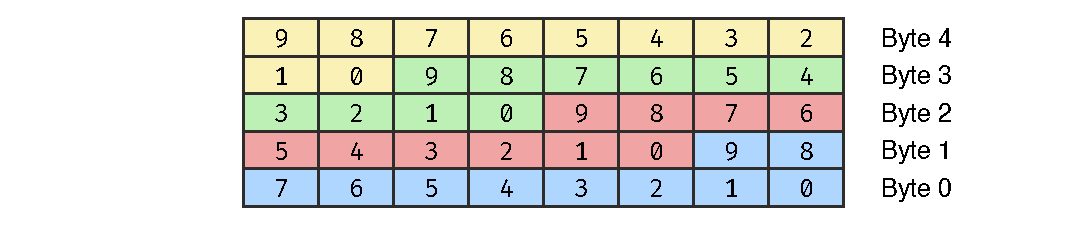
\includegraphics[width=\textwidth]{figures/unpacking/layout_10p_be.pdf}
    \caption{More intuitive visualization of little endness bit ordering.}
    \label{fig:mono10p_reordered}
\end{figure}
